% !TEX root = /Users/Gela/Desktop/Thesis_latex/thesis.tex

\section{Reverse Osmosis Membrane}
The membrane used is a reverse osomosis membrane manufactured by the DOW chemicals company. It is a custom made membrane for Baxter AB. 

\section{Pumps}
The pumps used in the system are magnet drive rotary vane pump TSSS401 from Fluid-o-Tech. They are designed to deliver a smooth flow reliably and optimized to reduce noise and power consumption. They are made for a maximum static pressure of 20 bar and has a speed limit of 1725 rpm. The nominal flow rate is 400 l/h. 

\section{Simscape/Simulink} 
\label{Simscape}

Simscape is a graphical programming tool within the Matlab simulink environment designed to model and simulate physical systems. A model of the RO-membrane and the flow path is designed using simscape and the simulated system could then be controlled using a control algorithm running in Simulink, a Matlab software too. The RO-membrane model encorporate separete mathematical models of the most important system dependencies, such as temperature , flow, pressure and conductivity.  

The system control is implemented in Simulink. 


\section{Speedgoat Real-Time Target Machine}
\label{speedgoat}
Speedgoat is a realtime target machine used for development. It is an FPGA I/O module with Simulink driver blocks. It is capable of simultaneous sampling and is used to drive the system rig. It contains an Intel 2.0 GHz quad core CPU. 

\begin{figure}[h]
    \centering
    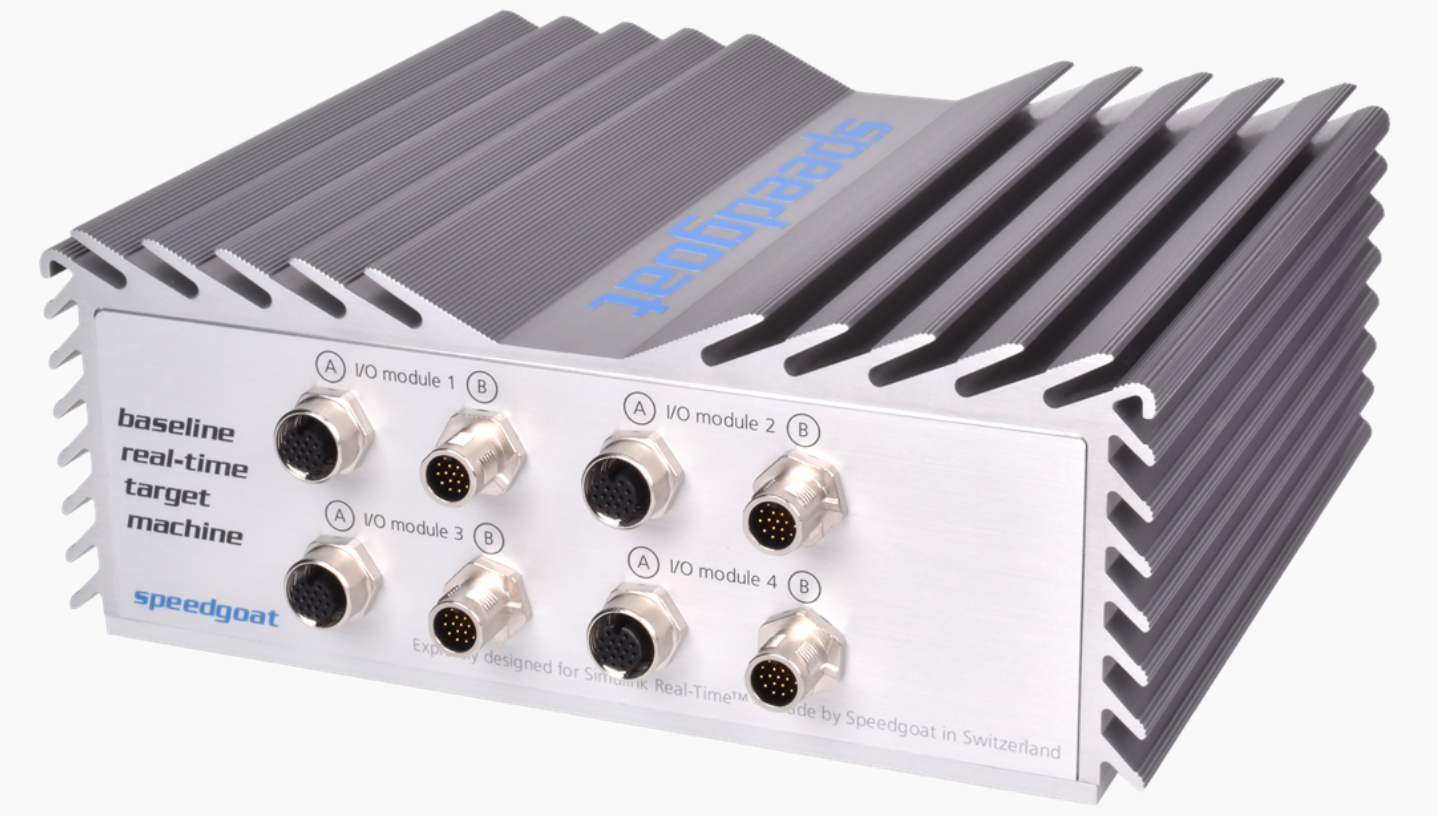
\includegraphics[width=0.4\textwidth]{Speedgoat}
    \caption{Speedgoat (Speedgoat real time simulation and testing, 2018)}
    \label{fig:speedgoat}
\end{figure}

\section{Measurement instruments} 
\label{measure}
Different instruments used to measure pressure, flow, temperature and conductivity in the physical rig.

\subsection{Conductivity sensor block}
\label{senscond}
A conductivity sensor block built by Gambro Lundia AB, called C3 is used to measure the water conductivity. In order to measure the required range two of the blocks where adjusted and calibrated. Two of the blocks, implemented in feed and recirculation path measures in range 0-3000 $\mu$S. The sensors cell implemented on permeate side measures up to 1500 $\mu$S.

\subsection{Temperature sensor}
\label{senstemp}
The C3 cell described in section \ref{senscond} contains sensors for temperature measurements and are used fro the temperature measurements in the system.

\subsection{Pressure sensor}
\label{senspress}
Pressure sensors where implemented in the C3 block, described in section \ref{senscond}, and calibrated in order to achieve the pressure at feed, recirculation and permeate side of the membrane. The pressure sensors range is between 0-20 bar.


\subsection{Flow meter}
\label{sensflow}
A flowsensor from Bronkhorst High-Tech B.V is used to measure the flow on permeate side. The flowmeter works in 4-1500 ml/min range and 0-100 bar with water as liquid flowing through. It has an accuracy of +- 1 ml/min. 

\begin{figure}[h]
    \centering
    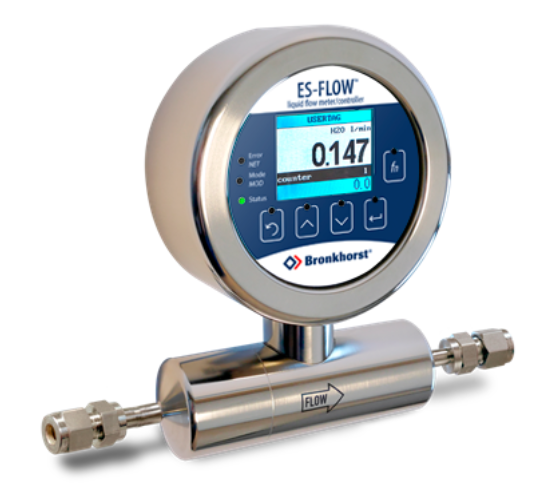
\includegraphics[width=0.4\textwidth]{Flowmeter}
    \caption{Flowmeter (BRONKHORST HIGH-TECH B.V.)}
    \label{fig:flowmeter}
\end{figure}









